\documentclass{article}
\usepackage[margin=1in]{geometry}
\usepackage{amsmath,amssymb}
\usepackage{parskip}
\usepackage{graphicx}
\usepackage{caption}
\usepackage{booktabs}
\DeclareMathOperator*{\argmin}{arg\,min}
\DeclareMathOperator*{\argmax}{arg\,max}

\title{CSE P 546 A - Homework 3}
\author{Thangakumar Dhanasekaran (2550520)}
\date{May-22-2026}

\begin{document}

\maketitle

\section*{A1}

\begin{enumerate}
  \item[(a)] \textbf{False.} Deep neural network loss functions are generally non-convex due to the composition of non-linear activations, so gradient descent can converge to a local minimum rather than the global optimum.

  \item[(b)] \textbf{False.} Initializing all weights to zero causes the symmetry problem: every neuron in a layer computes identical outputs and gradients, so they all update identically and the network never learns differentiated features. Random initialization breaks this symmetry.

  \item[(c)] \textbf{True.} Without non-linear activations, any composition of linear layers reduces to a single linear transformation, which can only learn linear decision boundaries. Non-linear activations are what allow the network to represent non-linear functions.

  \item[(d)] \textbf{False.} The backward pass traverses the same computation graph as the forward pass, so its time complexity is comparable (roughly $2\times$--$3\times$ the forward pass cost). It is not prohibitively larger.

  \item[(e)] \textbf{False.} Neural networks have high capacity but require large amounts of data and compute, and can be difficult to interpret. Simpler models (e.g., linear models, decision trees) are often preferable in low-data, resource-constrained, or interpretability-critical settings.
\end{enumerate}

\section*{A2}

\textbf{Claim.} For the feature map $\phi(x)$ whose $i$th component is
\[
  \phi_i(x) = \frac{1}{\sqrt{i!}}\,e^{-x^2/2}\,x^i, \quad i = 0, 1, 2, \ldots,
\]
the inner product satisfies $\phi(x)\cdot\phi(x') = e^{-(x-x')^2/2}$.

\begin{proof}
Compute the inner product directly by summing over all components $i \ge 0$:
\begin{align*}
  \phi(x)\cdot\phi(x')
  &= \sum_{i=0}^{\infty} \phi_i(x)\,\phi_i(x') \\
  &= \sum_{i=0}^{\infty}
       \left(\frac{1}{\sqrt{i!}}\,e^{-x^2/2}\,x^i\right)
       \left(\frac{1}{\sqrt{i!}}\,e^{-x'^2/2}\,x'^i\right) \\
  &= \sum_{i=0}^{\infty} \frac{1}{i!}\,e^{-(x^2+x'^2)/2}\,(xx')^i \\
  &= e^{-(x^2+x'^2)/2} \sum_{i=0}^{\infty} \frac{(xx')^i}{i!}.
\end{align*}

By the Taylor expansion $e^z = \displaystyle\sum_{i=0}^{\infty}\frac{z^i}{i!}$
applied with $z = xx'$, the sum equals $e^{xx'}$.  Therefore,
\begin{align*}
  \phi(x)\cdot\phi(x')
  &= e^{-(x^2+x'^2)/2}\cdot e^{xx'} \\
  &= e^{-(x^2 - 2xx' + x'^2)/2} \\
  &= e^{-(x-x')^2/2}.
\end{align*}

Hence $K(x,x') = e^{-(x-x')^2/2}$ is a valid kernel for $\phi$.
\end{proof}

\section*{A3}

\subsection*{Part a — Optimal hyperparameters (LOO cross-validation on $n=30$)}

\begin{center}
\begin{tabular}{lll}
\toprule
Kernel & $\lambda$ & Kernel parameter \\
\midrule
RBF      & $2.21 \times 10^{-3}$ & $\gamma = 10.54$ (median heuristic) \\
Polynomial & $3.73 \times 10^{-5}$ & $d = 16$ \\
\bottomrule
\end{tabular}
\end{center}

\subsection*{Part b — Predictions on a fine grid}

\begin{figure}[h]
  \centering
  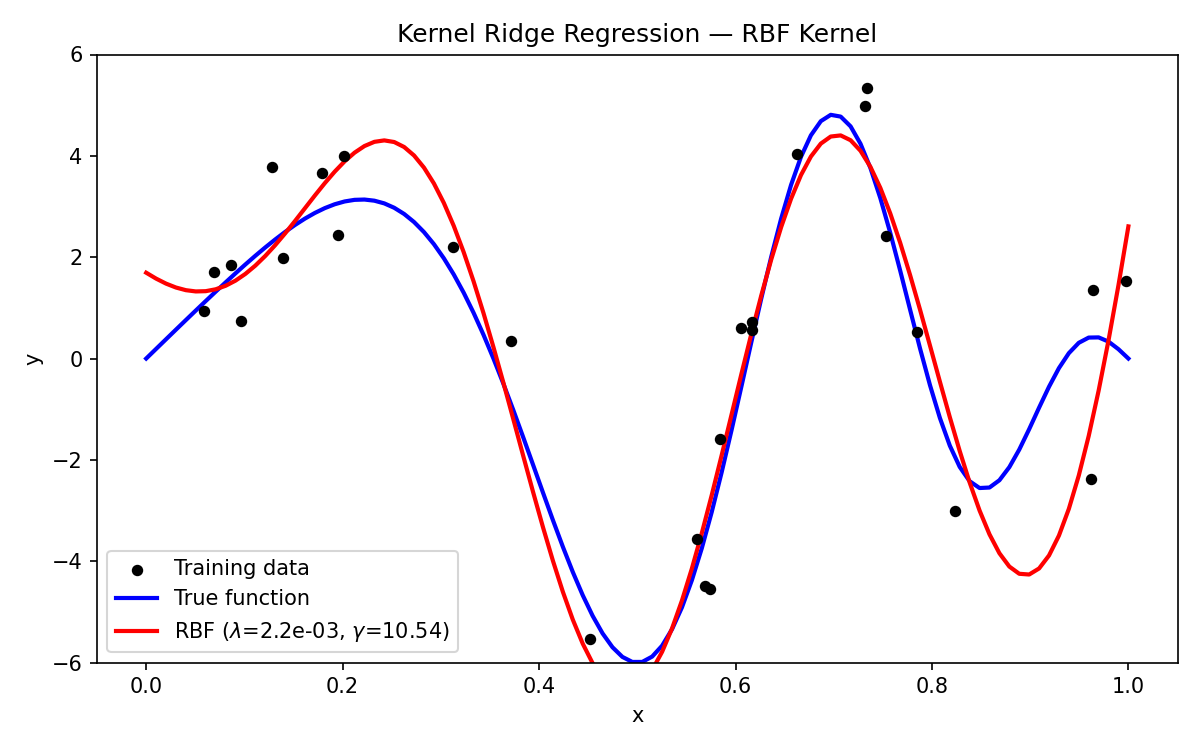
\includegraphics[width=0.85\textwidth]{a3_rbf_prediction.png}
  \caption{Kernel ridge regression with RBF kernel
    ($\lambda = 2.21\times10^{-3}$, $\gamma = 10.54$) trained on $n=30$ points.
    The red curve is the learned predictor; blue is the true function
    $f(x) = 6\sin(\pi x)\cos(4\pi x^2)$.}
\end{figure}

\begin{figure}[h]
  \centering
  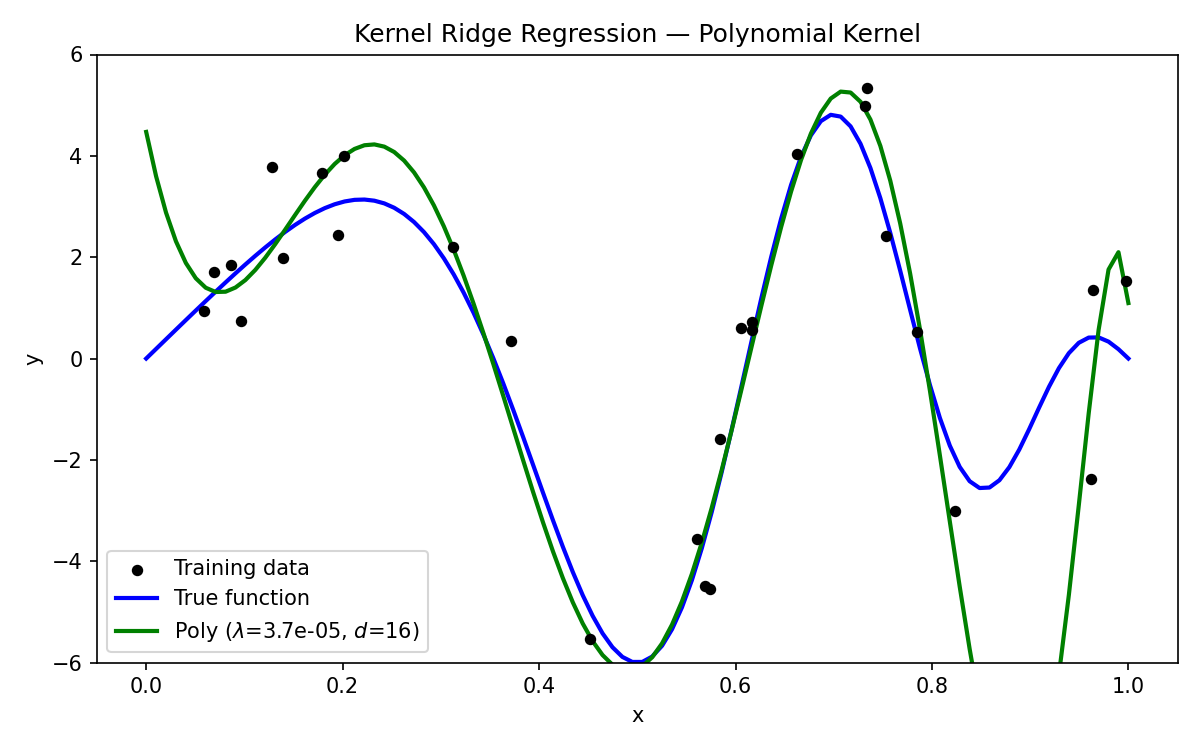
\includegraphics[width=0.85\textwidth]{a3_poly_prediction.png}
  \caption{Kernel ridge regression with polynomial kernel
    ($\lambda = 3.73\times10^{-5}$, $d = 16$) trained on $n=30$ points.
    The green curve is the learned predictor; blue is the true function.}
\end{figure}

\clearpage

\end{document}